%% LyX 2.2.4 created this file.  For more info, see http://www.lyx.org/.
%% Do not edit unless you really know what you are doing.
\documentclass[english]{article}
\usepackage{lmodern}
\usepackage[T1]{fontenc}
\usepackage[latin9]{inputenc}
\usepackage{geometry}
\geometry{verbose,tmargin=3cm,bmargin=3cm,lmargin=2.5cm,rmargin=2.5cm}
\usepackage{textcomp}
\usepackage{amstext}
\usepackage{amsmath}
\usepackage{amssymb}
\usepackage{graphicx}

\makeatletter

%%%%%%%%%%%%%%%%%%%%%%%%%%%%%% LyX specific LaTeX commands.
%% Because html converters don't know tabularnewline
\providecommand{\tabularnewline}{\\}

\makeatother

\usepackage{babel}
\begin{document}

\title{3F8: Inference\\
 Short Lab Report}

\author{Jaehyung Choi}
\maketitle
\begin{abstract}
This report applies logistic regression to a 2D binary classification
task, fitting parameters via gradient ascent of the log-likelihood.
We compare a linear model (test LL $\approx-0.629$) against non-linear
models that use Gaussian RBF feature expansions with widths $l\in\{0.01,0.1,1\}$.
The width $l=0.1$ gives the best test performance (LL $\approx-0.419$),
while $l=0.01$ fails to converge and $l=1$ overfits slightly relative
to $l=0.1$ but still improves over the linear baseline.
\end{abstract}

\section{Introduction}

Logistic regression models the probability of a binary label
$y\in\{0,1\}$ given input $\mathbf{x}\in\mathbb{R}^{2}$ as
$p(y=1\mid\mathbf{x})=\sigma(\beta^{\top}\tilde{\mathbf{x}})$,
where $\sigma$ is the logistic sigmoid and $\tilde{\mathbf{x}}$
is $\mathbf{x}$ with a prepended~1 (bias). Parameters $\beta$ are
found by gradient ascent on the log-likelihood.

A linear model can only produce straight decision boundaries, so when
the data is not linearly separable we might do better with richer
features. Here we replace the raw 2D inputs with Gaussian radial
basis function (RBF) features centred on the training points and compare
the effect of three kernel widths $l\in\{0.01,0.1,1\}$ on test
log-likelihood and classification accuracy.

\section{Exercise a)\label{sec:Exercise-a}}

The log-likelihood for logistic regression over $N$ data points is
\[
\mathcal{L}(\beta)=\sum_{n=1}^{N}\left[y^{(n)}\log\sigma\!\left(\beta^{\top}\tilde{x}^{(n)}\right)+(1-y^{(n)})\log\!\left(1-\sigma\!\left(\beta^{\top}\tilde{x}^{(n)}\right)\right)\right].
\]
To differentiate, we use the identities
$\frac{d}{dz}\log\sigma(z)=1-\sigma(z)$ and
$\frac{d}{dz}\log(1-\sigma(z))=-\sigma(z)$, which give
\[
\frac{\partial\log\sigma(\beta^{\top}\tilde{x}^{(n)})}{\partial\beta}
  =\bigl(1-\sigma(\beta^{\top}\tilde{x}^{(n)})\bigr)\tilde{x}^{(n)},
\quad
\frac{\partial\log(1-\sigma(\beta^{\top}\tilde{x}^{(n)}))}{\partial\beta}
  =-\sigma(\beta^{\top}\tilde{x}^{(n)})\tilde{x}^{(n)}.
\]
Multiplying each term by $y^{(n)}$ or $(1-y^{(n)})$ and summing:
\[
\frac{\partial\mathcal{L}(\beta)}{\partial\beta}
=\sum_{n=1}^{N}\!\bigl(y^{(n)}-\sigma(\beta^{\top}\tilde{x}^{(n)})\bigr)\tilde{x}^{(n)}
=\tilde{\mathbf{X}}^{\top}\!\bigl(\mathbf{y}-\sigma(\tilde{\mathbf{X}}\beta)\bigr)\,,
\]
where $\tilde{\mathbf{X}}$ is the $N\times(D{+}1)$ design matrix
with rows $\tilde{x}^{(n)\top}$ and $\sigma(\cdot)$ acts element-wise.

\section{Exercise b)}

Vectorised pseudocode for gradient ascent:
\begin{verbatim}
Function estimate_parameters(X, y, eta, T):

   Input:  N x D feature matrix X, N-vector y,
           learning rate eta, number of steps T
   Output: (D+1)-vector beta

   X_tilde <- prepend column of 1s to X     # N x (D+1)
   beta    <- random initialisation

   for i = 1 to T:
       s    <- sigmoid(X_tilde @ beta)       # N-vector
       grad <- X_tilde^T @ (y - s)           # (D+1)-vector
       beta <- beta + eta * grad

   return beta
\end{verbatim}
We set $\eta=1/N$ (here $1/800$). Dividing by $N$ keeps the effective
step size independent of dataset size. To check convergence we plot
the average log-likelihood at each step for both training and test sets.

\section{Exercise c)}

Figure \ref{fig:data_visualisation} shows the dataset. The two classes
(red and blue) overlap in the middle of the input space, so a linear
boundary will inevitably misclassify some points. This motivates trying
non-linear features later.

\begin{figure}
\begin{centering}
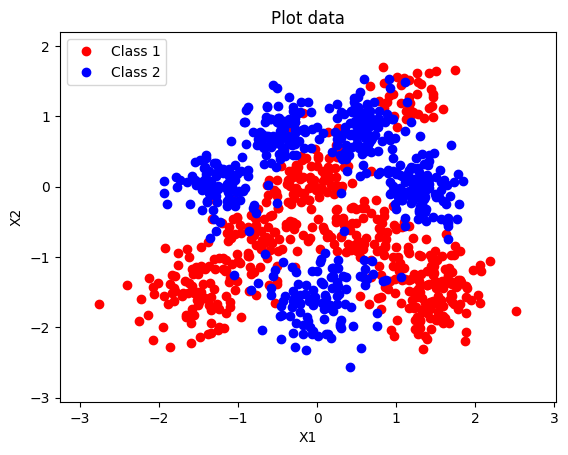
\includegraphics[width=0.3\paperwidth]{fig_data}
\par\end{centering}
\caption{Visualisation of the data.\label{fig:data_visualisation} }
\end{figure}


\section{Exercise d)}

We split the 1000 points into 800 training and 200 test. The gradient
update in Python is:
\begin{verbatim}
sigmoid_value = predict(X_tilde_train, w)
w = w + alpha * np.dot((y_train - sigmoid_value), X_tilde_train)
\end{verbatim}
With $\eta=1/800$ and 100 steps, the training and test log-likelihoods
(Figure~\ref{fig:learning_curves}) both rise sharply in the first
$\sim$20 steps and flatten out by step $\sim$50. The two curves
stay close together throughout, so overfitting is not an issue here.

The contour plot (Figure~\ref{fig:lin_contour}) confirms a straight
decision boundary at $p=0.5$, cutting through the overlap region.

\begin{figure}
\begin{centering}
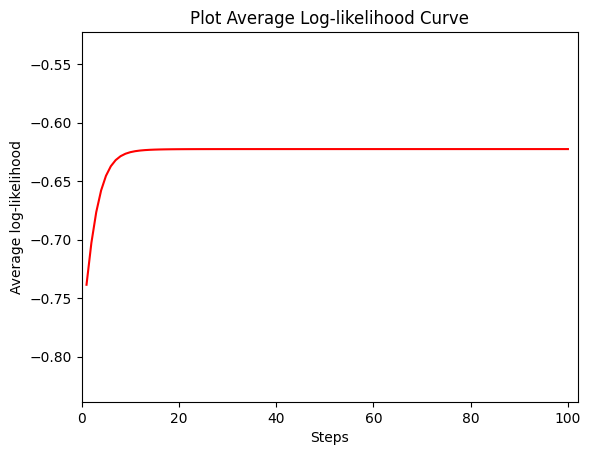
\includegraphics[width=0.3\paperwidth]{fig_lin_ll_train}\hspace{1cm}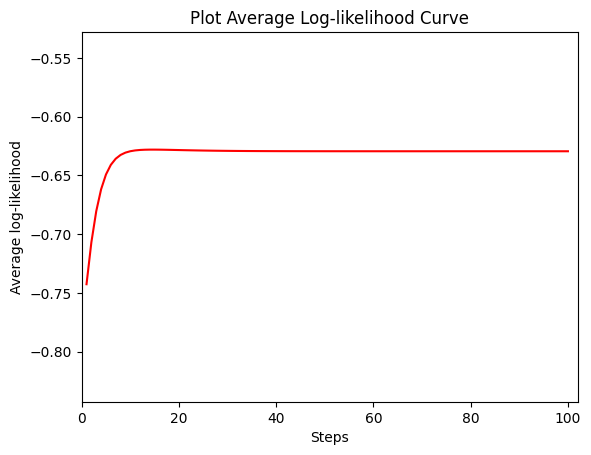
\includegraphics[width=0.3\paperwidth]{fig_lin_ll_test}
\par\end{centering}
\caption{Learning curves for the linear classifier: training (left) and
test (right) average log-likelihood.\label{fig:learning_curves} }
\end{figure}

\begin{figure}
\begin{centering}
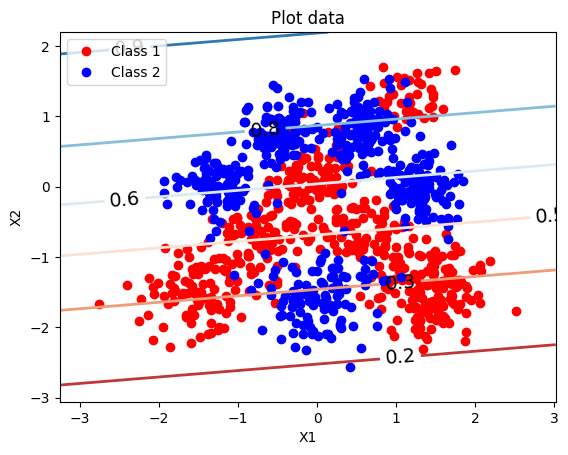
\includegraphics[width=0.3\paperwidth]{fig_lin_contour}
\par\end{centering}
\caption{Contour plot of the linear classifier's predictive probabilities.\label{fig:lin_contour} }
\end{figure}


\section{Exercise e)}

Table~\ref{tab:average_ll} gives the converged log-likelihoods.
The gap between train ($-0.6225$) and test ($-0.6294$) is small,
consistent with the learning curves in Figure~\ref{fig:learning_curves}.

The confusion matrix (Table~\ref{tab:confusion_test}) shows the model
gets 68\% of Class~0 and 76\% of Class~1 correct. The relatively
high false-positive rate (32\%) reflects the overlap visible in
Figure~\ref{fig:data_visualisation} --- points from both classes sit
on the wrong side of the linear boundary.

\begin{table}
\centering{}%
\begin{minipage}[t]{0.49\columnwidth}%
\begin{center}
\begin{tabular}{c|c}
\textbf{Avg. Train ll} & \textbf{Avg. Test ll}\tabularnewline
\hline
$-0.6225$ & $-0.6294$\tabularnewline
\hline
\end{tabular}
\par\end{center}
\caption{Average log-likelihoods for the linear classifier.\label{tab:average_ll}}
%
\end{minipage}%
\begin{minipage}[t]{0.49\columnwidth}%
\begin{center}
\begin{tabular}{cc|c|c}
 & \multicolumn{1}{c}{} & \multicolumn{1}{c}{$\hat{y}$} & \tabularnewline
 &  & 0 & 1\tabularnewline
\cline{2-4}
$y$ & 0 & $0.6818$ & $0.3182$\tabularnewline
\cline{2-4}
 & 1 & $0.2444$ & $0.7556$\tabularnewline
\cline{2-4}
\end{tabular}
\par\end{center}
\caption{Confusion matrix on the test set.\label{tab:confusion_test}}
%
\end{minipage}
\end{table}


\section{Exercise f)}

We expand the inputs using Gaussian RBF features centred on the 800
training points, with widths $l\in\{0.01,0.1,1\}$. Learning rates
were set to $\eta=0.01/800$, $0.1/800$, $0.5/800$ respectively,
with 1000, 1000, and 500 gradient steps. The contour plots are shown
in Figure~\ref{fig:contours_l}.

For $l=0.01$ (left), the basis functions are so narrow that the
feature matrix is nearly sparse --- each training point only activates
its own basis function. The gradients end up very small and the model
barely moves from its initialisation in 1000 steps; the contour plot
shows no meaningful decision boundary. For $l=0.1$ (middle), the
boundary is smooth and curved, fitting the shape of the class overlap
better than a straight line. For $l=1$ (right), the broad basis
functions overlap heavily, so the boundary is smoother but still
noticeably non-linear; it roughly follows the shape of the $l=0.1$
boundary but with less detail.

\begin{figure}
\begin{centering}
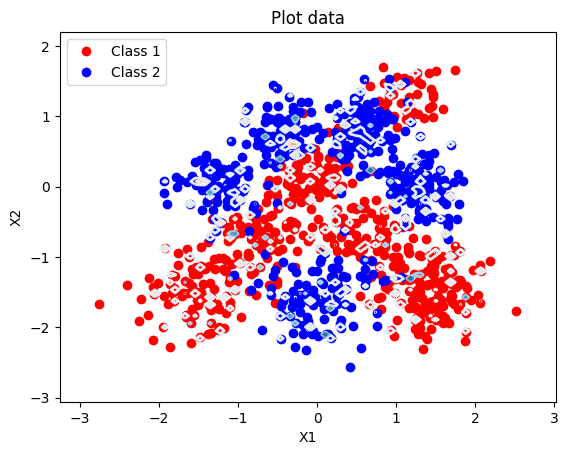
\includegraphics[width=0.32\textwidth]{fig_rbf001_contour}\hspace{0.15cm}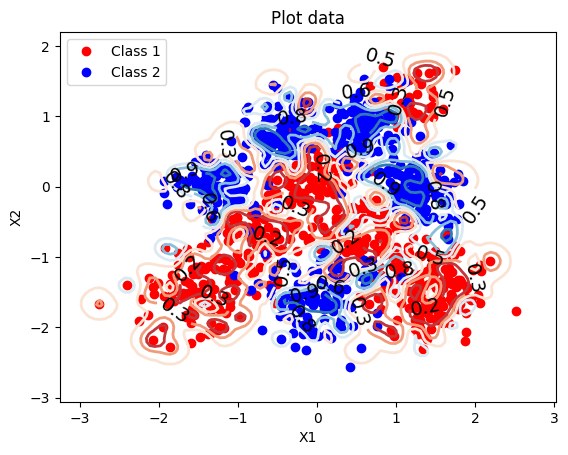
\includegraphics[width=0.32\textwidth]{fig_rbf01_contour}\hspace{0.15cm}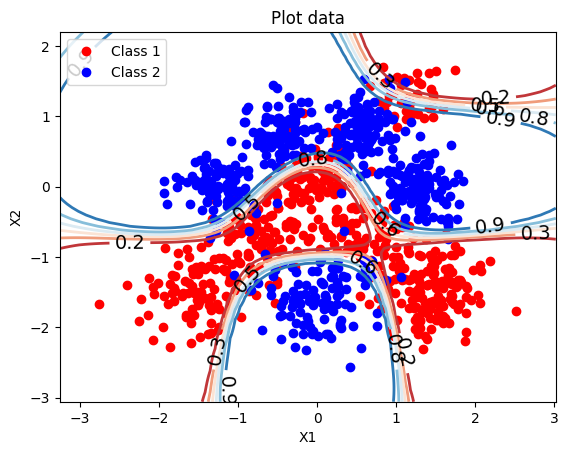
\includegraphics[width=0.32\textwidth]{fig_rbf1_contour}
\par\end{centering}
\caption{Contours of the class predictive probabilities for $l=0.01$ (left),
$l=0.1$ (middle), $l=1$ (right).\label{fig:contours_l} }
\end{figure}


\section{Exercise g)}

Tables~\ref{tab:avg_ll_l_001}--\ref{tab:avg_ll_l_1} show the final
log-likelihoods. The $l=0.01$ model has not converged: both its
train ($-0.796$) and test ($-0.700$) log-likelihoods are worse
than the linear model, consistent with the degenerate contour plot.
The $l=0.1$ model achieves the best test LL ($-0.419$). The $l=1$
model has the lowest (best) training LL ($-0.320$) but its test LL
($-0.497$) is worse than $l=0.1$; the gap of $0.177$ between train
and test indicates it is starting to overfit, even though it still
outperforms the linear baseline ($-0.629$) on test.

The confusion matrices (Tables~\ref{tab:conf_l_001}--\ref{tab:conf_l_1})
tell a similar story. For $l=0.01$, the model predicts Class~1
for nearly everything (FP$=0.96$), confirming it has not learned
anything useful. For $l=0.1$, both classes are classified at about
82\% accuracy, a clear step up from the linear model (68\%/76\%).
For $l=1$, Class~1 accuracy (81\%) is similar to $l=0.1$, but
Class~0 (``true negative'') sits at 98\% --- the model is somewhat
biased toward predicting Class~1. Overall, both $l=0.1$ and $l=1$
beat the linear model, with $l=0.1$ giving the best balance between
the two classes and the highest test log-likelihood.

\begin{table}
\centering{}%
\begin{minipage}[t]{0.3\textwidth}%
\begin{center}
\begin{tabular}{c|c}
\textbf{Avg. Train ll} & \textbf{Avg. Test ll}\tabularnewline
\hline
$-0.7957$ & $-0.7003$\tabularnewline
\hline
\end{tabular}\caption{Results for $l=0.01$\label{tab:avg_ll_l_001}}
\par\end{center}%
\end{minipage}\hspace{0.5cm}%
\begin{minipage}[t]{0.3\textwidth}%
\begin{center}
\begin{tabular}{c|c}
\textbf{Avg. Train ll} & \textbf{Avg. Test ll}\tabularnewline
\hline
$-0.4597$ & $-0.4187$\tabularnewline
\hline
\end{tabular}\caption{Results for $l=0.1$\label{tab:avg_ll_l_01}}
\par\end{center}%
\end{minipage}\hspace{0.5cm}%
\begin{minipage}[t]{0.3\textwidth}%
\begin{center}
\begin{tabular}{c|c}
\textbf{Avg. Train ll} & \textbf{Avg. Test ll}\tabularnewline
\hline
$-0.3203$ & $-0.4971$\tabularnewline
\hline
\end{tabular}\caption{Results for $l=1$\label{tab:avg_ll_l_1}}
\par\end{center}%
\end{minipage}
\end{table}

\begin{table}
\centering{}%
\begin{minipage}[t]{0.33\textwidth}%
\begin{center}
\begin{tabular}{cc|c|c}
 & \multicolumn{1}{c}{} & \multicolumn{1}{c}{$\hat{y}$} & \tabularnewline
 &  & 0 & 1\tabularnewline
\cline{2-4}
$y$ & 0 & $0.0364$ & $0.9636$\tabularnewline
\cline{2-4}
 & 1 & $0.1333$ & $0.8667$\tabularnewline
\cline{2-4}
\end{tabular}
\par\end{center}
\caption{Conf. matrix $l=0.01$.\label{tab:conf_l_001}}
%
\end{minipage}%
\begin{minipage}[t]{0.33\textwidth}%
\begin{center}
\begin{tabular}{cc|c|c}
 & \multicolumn{1}{c}{} & \multicolumn{1}{c}{$\hat{y}$} & \tabularnewline
 &  & 0 & 1\tabularnewline
\cline{2-4}
$y$ & 0 & $0.8182$ & $0.1818$\tabularnewline
\cline{2-4}
 & 1 & $0.1778$ & $0.8222$\tabularnewline
\cline{2-4}
\end{tabular}
\par\end{center}
\caption{Conf. matrix $l=0.1$.\label{tab:conf_l_01}}
%
\end{minipage}%
\begin{minipage}[t]{0.33\textwidth}%
\begin{center}
\begin{tabular}{cc|c|c}
 & \multicolumn{1}{c}{} & \multicolumn{1}{c}{$\hat{y}$} & \tabularnewline
 &  & 0 & 1\tabularnewline
\cline{2-4}
$y$ & 0 & $0.8091$ & $0.1909$\tabularnewline
\cline{2-4}
 & 1 & $0.0222$ & $0.9778$\tabularnewline
\cline{2-4}
\end{tabular}
\par\end{center}
\caption{Conf. matrix $l=1$.\label{tab:conf_l_1}}
%
\end{minipage}
\end{table}


\section{Conclusions}

The linear classifier converges quickly and gives a train/test LL of
$-0.623$/$-0.629$ with no sign of overfitting, but misclassifies
a substantial fraction of both classes due to the non-linear overlap
in the data.

RBF feature expansion can improve on this, but the kernel width $l$
matters a lot. With $l=0.01$ the features are too sparse for gradient
ascent to make progress at a reasonable learning rate. With $l=0.1$
we get the best test LL ($-0.419$) and balanced accuracy ($\sim$82\%
on both classes). With $l=1$ the model still outperforms the linear
baseline on test, but overfits more than $l=0.1$ (train--test gap of
$0.177$ vs $0.041$) and is biased toward predicting Class~1.
In practice, $l$ should be chosen by monitoring test performance.

\end{document}
